\chapter{MIP Approach}
\label{chapter-mip}

In this chapter we introduce a new approach to finding maximum ID sets. First, we transform the problem formulation to maximum weighted IS problem formulation. Then we transform this into an MIP formulation, and demonstrate how this can be solved using a solver such as GLPK \cite{glpk}. \nomenclature{GLPK}{GNU Linear Programming Kit}
We will continue by~applying heuristic approaches to improve the performance of the process.

\section{ID Set to IS Formulation}

Given $C = \{m_1, \ldots, m_n\}$ a set of all AMs in a document, we construct a graph $G = (V,E)$ as follows. For each AM $m_i \in C$ we create a vertex $v_{name(m_i)}$. Two vertices $v_{name(m_i)}$ and $v_{name(m_j)}$ shall be connected by an edge iff they cannot share the same ID set, either because they have the same type ($\tau(m_i) = \tau(m_j)$), or their images intersect ($\iota(m_i) \cap \iota(m_j) \neq \emptyset$). Weight of a vertex $v_{name(m_i)}$ is the weight of the attribute mapping: $w(v_{name(m_i)}) = weight(m_i)$.

Now finding the maximum weighted IS in $G$ finds the maximum (optimal) ID set in the original document.

\section{IS to MIP Formulation}

Given a~graph $G = (V,E)$ with a~weight function $w: V \rightarrow \mathbb{R}$, we introduce a~binary variable $x_i$ for each vertex $v_i \in V$ and an~inequality constraint $x_i + x_j \leq 1$ for each edge $e = (v_i, v_j) \in E$. Furthermore we introduce an~objective function in~form $\sum_{x_i} x_i w(v_i)$.

It is obvious that the objective function and all the constraints consitute a~MIP instance, and that solving it finds the maximum weigthed IS in $G$.

\section{Finding ID Sets With GLPK}
\label{section-mip-glpk}

By chaining these two translations we can create a MIP formulation for a given set of AMs from a document. Solving this MIP instance will give us the optimal ID set for this document.

GLPK is a multi-platform, multi-purpose solver well suited for this task. It~uses the Simplex method to solve LP problems and \textit{Branch \& Bound} for MIP. 

\paragraph{\textit{Branch \& Bound}} This is an optimization method where the search space is~systematically divided into smaller sub-spaces. This is the \textit{branching} component, and a so-called \textit{search tree} is built this way. Then, the sub-problems are recursively solved and whole branches of the search tree are discarded when it becomes obvious that the solution does not lie there. This is the \textit{bounding} component. See \cite{land60a} for detailed description.\\

An advantage of using \textit{Branch \& Bound} is~that while traversing the search tree it finds intermittent, sub-optimal solutions. It is thus possible to limit the~total search time and instead of the optimum take the best solution found so far.\\

We will now demonstrate the full process of~finding the optimal ID set of~an~example XML file using GLPK.

\subsection*{Example}

Consider again our XML file fragment.

\begin{verbatim}
<x>
  <y a="1" b="2"/>
  <y a="3" c="4"/>
  <y/>
  <z a="1"/>
</x>
\end{verbatim}

Recall that attribute mappings in this example are $C = \{M_{y}^{a}, M_{y}^{b}, M_{y}^{c}, M_{z}^{a}\}$. Corresponding vertices in the IS formulation will be $V = \{v_{y-a}, v_{y-b}, v_{y-c}, v_{z-a}\}$. Edges in the IS formulation will be the following ones:

\begin{eqnarray*}
(v_{y-a},v_{y-b}), \\
(v_{y-a},v_{y-c}), \\
(v_{y-b},v_{y-c}), \\
(v_{y-a},v_{z-a}). \\
\end{eqnarray*}

The first three edges are due to the type collision ($y$), the last one is due to~$\iota(M_{y}^{a}) \cap \iota(M_{z}^{a}) = \{1\}$. The graph $G$ constructed in this way is shown in~Figure~\ref{image-mip-is-graph}.

\begin{figure}
  \caption{IS Representation Graph}
  \label{image-mip-is-graph}
  \centering
	 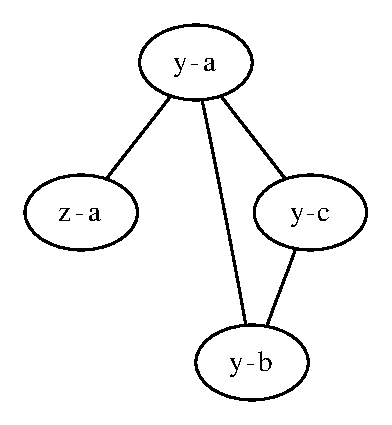
\includegraphics[width=.25\textwidth]{images/is-representation}
\end{figure}

The next step is the MIP formulation. We do not need to translate from the IS formulation, as the translation from ID set formulation is straightforward, too. For each AM $m$ there will be one binary variable $x_{name(m)}$. Objective function coefficients in vector $\mathbf{c}$ will be weights of respective mappings. For each pair of~AMs $m_1, m_2$ that cannot share the same ID set there shall be a row in matrix $A$ representing the inequality $x_{name(m_1)} + x_{name(m_2)} \leqslant 1$. $\mathbf{b}$ will be a vector of~ones of corresponding length.

\[
\mathbf{x} =
\begin{bmatrix}
x_{y-a} \\
x_{y-b} \\
x_{y-c} \\
x_{z-a} \\
\end{bmatrix},
\mathbf{c} = 
\begin{bmatrix}
weight(M_{y}^{a}) \\
weight(M_{y}^{b}) \\
weight(M_{y}^{c}) \\
weight(M_{z}^{a}) \\
\end{bmatrix} =
\begin{bmatrix}
0.2 \\
0.2 \\
0.6 \\
0.4 \\
\end{bmatrix},
\mathbf{b} =
\begin{bmatrix}
1 \\
1 \\
1 \\
1 \\
\end{bmatrix},
A =
\begin{pmatrix}
0 & 1 & 1 & 0 \\
1 & 0 & 1 & 0 \\
1 & 1 & 0 & 0 \\
1 & 0 & 0 & 1 \\
\end{pmatrix}
\]

The problem now is, recall, to solve the following:

\begin{eqnarray*}
\max_{x} z & = & \mathbf{c}^{\mathrm{T}}\mathbf{x} \\
s.t.\, A\mathbf{x} & \leqslant & \mathbf{b}. \\
\end{eqnarray*}

In GLPK \textit{MathProg} language \cite{mathprog}, this translates to the following.

\begin{scriptsize}
\begin{verbatim}
set AMs;
param Weight {i in AMs};
var x {i in AMs} binary;
maximize z: sum {i in AMs} x[i] * Weight[i];
s.t. c1: x['y-a'] + x['y-b'] <= 1;
s.t. c2: x['y-a'] + x['y-c'] <= 1;
s.t. c3: x['y-b'] + x['y-c'] <= 1;
s.t. c4: x['y-a'] + x['z-a'] <= 1;
data;
set AMs := y-a y-b y-c z-a;
param Weight :=
y-a 0.6
y-b 0.2
y-c 0.2
z-a 0.4;
end;
\end{verbatim}
\end{scriptsize}

We can use this as an input for the GLPK solver, and we get the solution.

\begin{scriptsize}
\begin{verbatim}
...
Problem:    glpk_input
Rows:       5
Columns:    4 (4 integer, 4 binary)
Non-zeros:  12
Status:     INTEGER OPTIMAL
Objective:  z = 0.6 (MAXimum)

...

   No. Column name       Activity     Lower bound   Upper bound
------ ------------    ------------- ------------- -------------
     1 x[y-a]       *              1             0             1 
     2 x[y-b]       *              0             0             1 
     3 x[y-c]       *              0             0             1 
     4 x[z-a]       *              0             0             1 

...
\end{verbatim}
\end{scriptsize}

This output tells us that the solution is $x_{y-a} = 1$, $x_{y-b} = 0$, $x_{y-c} = 0$ and $x_{z-a} = 0$. This means that the optimal ID set with maximum weight contains only the $M_{y}^{a}$ attribute mapping.\\

It is obvious that this approach works and for any possible input we can let GLPK find the optimal solution. However, sometimes it takes too long to find the optimum (see e.g. Section \ref{section-glpk-comparison}), hence, the aim of this work is to improve this process.

\section{Heuristics}
\label{section-mip-heuristics}

The definition of \textit{heuristic} or \textit{heuristic algorithm} varies from one source to another. We shall be using it roughly in the following sense.

\begin{define}[Heuristic]
	A \textit{heuristic} is an approach to problem solving based on prior experience, educated guess or common knowledge.
\end{define}

\begin{define}[Heuristic Algorithm]
	A \textit{heuristic algorithm} is one that, in a reasonably short time, generates a good, maybe even optimal solution to an optimization problem. However, it will not provide any formal guarantee about its quality.
\end{define} 

This definion of heuristic algorithm coming from \cite{heu-lecture} is rather vague, however, it will be sufficient for us.

An example of a heuristic is the commonly used approach of \textit{trial and error}: after a failed attempt, change some parameter and try again. We will see many more heuristics later in this chapter.

While a heuristic algorithm can be seen as a tool designed to solve one specific problem, the notion of a \textit{metaheuristic} reminds of a recipe to solve a whole family of problems. We shall be using the metaheuristic presented in Figure \ref{image-metaheuristic} to find optimal ID sets in this work. But before we start describing its structure and components, we need to introduce some more notions.

\begin{figure}
  \caption{Metaheuristic schema}
  \label{image-metaheuristic}
  \centering
    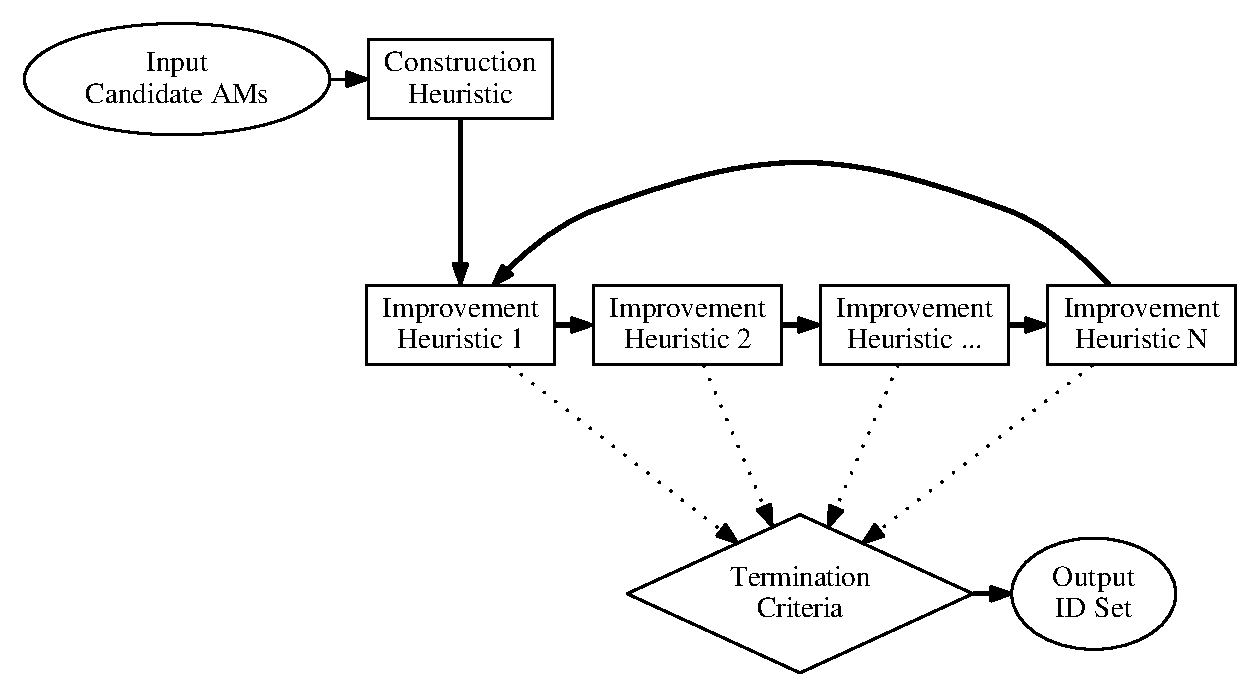
\includegraphics[width=\textwidth]{images/metaheuristic}
\end{figure}

\begin{define}[Solution Space, Solution Quality]
	Solution space in general is~the~set of all permissible solutions (not violating any constraints). In the specific case of a MIP formulation it is the set of all $\mathbf{x}$ subject to $A\mathbf{x} \leqslant \mathbf{b}$. Every solution in the solution space has its \textit{quality}, in case of MIP for solution $\mathbf{x}$ it~is~the value of the objective function in $\mathbf{x}$.
\end{define}

\begin{define}[Solution Neighborhood]
	Neighborhood of a solution $\mathbf{x}$ in~the~solution space are all the other solutions close to~$\mathbf{x}$ according to~some metric.
\end{define}

The precise definition of the neighborhood is always adjusted according to~specific needs. However, the neighborhood should be defined so that is \textit{continuous} (with respect to quality) to be useful. The exact reasons for this requirement are sketched in Section \ref{section-mip-ihs}.

\begin{define}[Solution Pool, Incumbent Solution]
	\textit{Solution pool} (sometimes called pool of feasible solutions or feasible pool) is a set of solutions of different qualities that were found in one of the stages of the metaheuristic. The solution(s) with the highest quality is (are) called the \textit{incumbent} solution(s).
\end{define}

A quick reminder of what we are trying to solve using our metaheuristic: given a list of AMs with weights, find a non-conflicting subset maximizing the sum of weights in the subset. This sum will henceforth be considered the quality of the solution (subset). We will now describe its structure, please refer again to Figure \ref{image-metaheuristic}.

First we take the list of candidate AMs and ask a \textit{construction heuristic} (see Section \ref{section-mip-chs}) to provide us with a pool of solutions. Then, in a loop, we use this pool as input for \textit{improvement heuristics} (see Section \ref{section-mip-ihs}) and in turns ask them to improve it. All the time we check whether \textit{termination criteria} are met, and if so, we terminate the metaheuristic. The incumbent solution from the last pool is then declared the Output ID set.\\

The notion of metaheuristic covers a wide range of topics in the field of~heuristics, such as Tabu Search (see \cite{Glover:1997:TS:549765}), Ant Colony Optimization (see \cite{dorigo2004ant}) or Genetic Algorithms (see e.g. \cite{goldberg1989genetic}), to name a few.\\

We will now introduce the heurisitics we have implemented to use in our metaheuristic for finding optimal ID sets.

\subsection{Constructions Heuristics}
\label{section-mip-chs}
\nomenclature{CH}{Construction Heuristic}

When we start to solve a problem using a metaheuristic approach, at first we have no solutions at all. The purpose of a construction heuristic (CH) is then to provide us with at least some solution. This may or may not be already the~optimum, in the latter case it will be improved on later using improvement heuristics (IH). Some IHs can profit from a pool of several sub-optimal solutions, and some CHs can produce this pool from them.

\subsubsection{\heu{FIDAX}}
\label{section-mip-fidax}

The first construction heuristic is the algorithm described in \cite{fidax} (we shall call it \heu{FIDAX} from now on). It can trivially be used to give us one feasible solution - it is, after all, a deterministic heuristic algorithm.

The algorithm works in two steps. First, all candidate AMs are grouped according to their types, and for each type the AM with the highest weight is~selected. Second, all these AMs (now called $C'$) are traversed in order of their decreasing size. For each AM $m$, a set $S$ of all conflicting AMs from $C'$ is found and weights of both $m$ and $S$ are calculated. Then the weights are compared and either $m$ or $S$ is removed from $C'$.

The pseudocode of this CH (taken from the original article with trivial modifications without changing the logic) is in Listing \ref{listing-ch-fidax}.

\begin{algorithm}
\caption{\heu{FIDAX} CH}
\label{listing-ch-fidax}
\begin{algorithmic}
\REQUIRE $C$ list of candidate AMs
\ENSURE a feasible solution
\STATE $C' \gets C$ sorted by decreasing size
\STATE Compute the weight $w(m)$ of each $m$ in $C$
\FORALL{$t$ in $\Sigma^E$}
  \STATE Let $m$ be a \textbf{highest-weight} mapping of type $t$ in $C'$
  \STATE Remove from $C'$ all mappings of type $t$ except $m$
\ENDFOR
\FORALL{$m$ in $C'$}
  \STATE $S \gets$ all mappings in $C'$ whose images intersect $\iota(m)$
  \IF{$w(m) > \sum_{p \in S} w(p)$}
    \STATE remove all $p \in S$ from $C'$
  \ELSE
    \STATE remove $m$ from $C'$
  \ENDIF
\ENDFOR
\RETURN $C'$
\end{algorithmic}
\end{algorithm}

\subsubsection{\heu{Random}}
\label{heu-ch-random}

One of the most natural heuristics when dealing with the ID set problem can be described as follows: select from candidate AMs at random, if possible (addition would not violate the ID set condition) add them to the solution. This is~obviously a greedy heuristic.

The advantages of this trivial heuristic are simplicity, speed and ease with which it can create a pool of variable solutions, almost for free. As we will see later in the experiments (Section \ref{section-experiments-random-fuzzy-fidax}), it performs surprisingly well.

See the Listing \ref{listing-ch-random} for its pseudocode.

\begin{algorithm}
\caption{\heu{Random} CH}
\label{listing-ch-random}
\begin{algorithmic}
\REQUIRE $N$ required size of pool
\REQUIRE $C$ list of candidate AMs
\ENSURE pool of $N$ feasible solutions
\STATE $r \gets $ empty pool
\FOR{$i = 1 \to N$}
  \STATE \COMMENT{create 1 solution}
  \STATE $s \gets $ empty solution
  \WHILE{$s$ is a feasible ID set}
    \STATE $a \gets $ pick at random from $C \backslash S$
    \STATE $s \gets s \cup a$
  \ENDWHILE
  \STATE $r \gets r \cup s$
\ENDFOR
\RETURN $r$
\end{algorithmic}
\end{algorithm}

\subsubsection{\heu{Fuzzy}}
\label{heu-ch-fuzzy}

\heu{Fuzzy} is an improvement over the \heu{Random} CH: the next AM to be added is~selected based on \textit{weighted} instead of uniform random. The weight used here is~the usual weight of an AM as defined in Section \ref{section-definitions-weight}. Because of the randomness involved in the choice, we can again easily create a pool of solutions this way.

This is again a greedy heuristic, the Listing \ref{listing-ch-fuzzy} contains its pseudocode.

\begin{algorithm}
\caption{\heu{Fuzzy} CH}
\label{listing-ch-fuzzy}
\begin{algorithmic}
\REQUIRE $N$ required size of pool
\REQUIRE $C$ list of candidate AMs
\ENSURE pool of $N$ feasible solutions
\STATE $r \gets $ empty pool
\FOR{$i = 1 \to N$}
  \STATE \COMMENT{create 1 solution}
  \STATE $s \gets $ empty solution
  \STATE $C' \gets C$

  \WHILE{$C' $ not empty}
    \STATE $a \gets $ pick at weighted random from $C'$
    \IF{$s \cup a$ is a feasible ID set}
      \STATE $s \gets s \cup a$
      \STATE $C' \gets C' \backslash a$
    \ENDIF
    \FORALL{$c \in C'$}
      \IF{$s \cup c $ is \textbf{not} a feasible ID set}
        \STATE \COMMENT {if $c$ cannot be possibly added anymore}
        \STATE $C' \gets C' \backslash c$
      \ENDIF
    \ENDFOR
  \ENDWHILE

  \STATE $r \gets r + s$
\ENDFOR
\RETURN $r$
\end{algorithmic}
\end{algorithm}

\subsubsection{\heu{Incremental}}

This trivial heuristic sorts all candidate AMs by their decreasing weights (see Section \ref{section-definitions-weight}) and then tries to iteratively add them to solution, if possible. This way it can create only one solution, and again, this is a greedy heuristic.

See Listing \ref{listing-ch-incremental} for its pseudocode.

\begin{algorithm}
\caption{\heu{Incremental} CH}
\label{listing-ch-incremental}
\begin{algorithmic}
\REQUIRE $C$ list of candidate AMs
\ENSURE a feasible solution
\STATE $C' \gets $ sort $C$ by decreasing weight
\STATE $s \gets $ empty solution
\FORALL{$c \in C'$}
  \IF{$s \cup c$ is a feasible ID set}
    \STATE $s \gets s + c$
  \ENDIF
\ENDFOR
\RETURN $s$
\end{algorithmic}
\end{algorithm}

\subsubsection{\heu{Removal}}

This is basically a reversal of the idea from the \heu{Incremental} heuristic - start with a solution containing all the candidate AMs. This probably does not satisfy the ID set condition. Therefore, sort them by increasing size and start removing them from the solution, until it satisfies the ID set condition. Again, this is a greedy heuristic returning only one solution.

See Listing \ref{listing-ch-removal} for its pseudocode.

\begin{algorithm}
\caption{\heu{Removal} CH}
\label{listing-ch-removal}
\begin{algorithmic}
\REQUIRE $C$ list of candidate AMs
\ENSURE a feasible solution
\STATE $C' \gets $ sort $C$ by increasing weight
\STATE $s \gets C'$
\FORALL{$c \in s$}
  \IF{$s$ is a feasible ID set}
    \RETURN $s$
  \ENDIF
  \STATE $s \gets s \backslash c$
\ENDFOR
\end{algorithmic}
\end{algorithm}

\subsubsection{Truncated Branch \& Bound - \heu{Glpk}}

This construction heuristic will be called \heu{Glpk} from now on. It is basically a~time-constrained run of GLPK. Recall that GLPK uses a the \textit{Branch \& Bound} algorithm that produces feasible solutions even before the optimum is found. Limiting the run time gives us the best solution found so far, which means this is a construction heuristic.

To be able to create a pool of solutions, the GLPK input in MathProg langauge is always randomly shuffled by changing the order in which variables and constraints appear. This is causes the solver to explore the search tree in~various orders, producing different solution in each of the time-constrained runs.

\subsection{Improvement Heuristics}
\label{section-mip-ihs}

\nomenclature{IH}{Improvement Heuristic}

Improvement heuristics in general start with a solution pool, attempt to improve one or more solutions in it and then return this improved pool in~the~end. We will need two notions to describe their behavior.

\paragraph{Intensification}

is the attempt to move the solution towards the nearby local optimum in~the~solution space.

\paragraph{Diversification}

is the attempt to move the solution away (escape) from the~local optimum, to be able to explore more of the solution space when the metaheuristic starts stagnating.\\

A metaheuristic needs to combine intensification and diversification tendencies to explore the solution space and at the same time arrive at a local optimum. Recall the requirement for the solution space to be continuous in~terms of quality: this guarantees that as we approach a solution $\mathbf{x}$, the quality of solutions we encounter approaches the quality of $\mathbf{x}$.

\subsubsection{\heu{Identity}}

This ultimately trivial improvement heuristic does nothing. It simply returns the feasible pool unchanged. For the sake of completeness, see its Listing \ref{listing-ih-identity}.

\begin{algorithm}
\caption{\heu{Identity} IH}
\label{listing-ih-identity}
\begin{algorithmic}
\REQUIRE $FP$ pool of feasible solutions
\ENSURE the same pool of feasible solutions
\RETURN $FP$
\end{algorithmic}
\end{algorithm}

\subsubsection{\heu{Remove Worst}}

This trivial IH tries to improve the solution pool by removing the worst solution (i.e. the one with the lowest quality). This is interesting in cooperation with other improvement heuristics that increase the solution pool size, to keep it~from growing by pruning inferior solutions.

See Listing \ref{listing-ih-removeworst} for details.

\begin{algorithm}
\caption{\heu{Remove Worst} IH}
\label{listing-ih-removeworst}
\begin{algorithmic}
\REQUIRE $FP$ pool of feasible solutions
\ENSURE pool of feasible solutions
\STATE $s_{min} \gets $ solution with the lowest weight $\in FP$
\RETURN $FP \backslash s_{min}$
\end{algorithmic}
\end{algorithm}

\subsubsection{\heu{Random Remove}}

This is again a rather trivial diversification improvement heuristic. By removing a random subset of specified size from each solution in the pool, it provides the variability needed to escape from local optima in the solution space.

The number of AMs to remove from each solution is specified as fraction from $(0, 1)$ of the solution size (number of AMs in solution). For example, \heu{Random Remove} with $fraction = 0.1$ would remove 1 random AM from a solution containing 10 AMs and 2 from a solution containing 17 AMs (due to~rounding).

This heuristic returns a pool of solutions of the same size as it got on input.

See Listing \ref{listing-ih-randomremove} for pseudocode.

\begin{algorithm}
\caption{\heu{Random Remove} IH}
\label{listing-ih-randomremove}
\begin{algorithmic}
\REQUIRE $FP$ pool of feasible solutions
\REQUIRE $k \in (0,1)$ fraction of AMs to remove from each $s \in FP$
\ENSURE pool of feasible solutions
\FORALL{$s \in FP$}
  \STATE $K \gets k * |s|$
  \STATE remove $K$ random AMs from $s$
\ENDFOR
\RETURN $FP$
\end{algorithmic}
\end{algorithm}

\subsubsection{\heu{Hungry}}

This simple improvement heuristic assumes that the solutions in the pool are not ``complete'', i.e. there are AMs that could be added to them without violating the ID set condition.

\heu{Hungry} tries to improve each solution in the feasible pool in the following way. It orders all candidate AMs not present in the solution by decreasing weight. Afterwards, it iteratively tries to extend the solution with these AMs, taking care not to violate the ID set condition. The resulting solution (whether any AMs were added or not) is then returned to the pool. This is then intensification, and Listing \ref{listing-ih-hungry} captures the process.\\

\begin{algorithm}
\caption{\heu{Hungry} IH}
\label{listing-ih-hungry}
\begin{algorithmic}
\REQUIRE $FP$ pool of feasible solutions
\REQUIRE $C$ list of candidate AMs
\ENSURE pool of feasible solutions
\FORALL{$s \in FP$}
  \STATE \COMMENT {improve a single solution}
  \STATE $C' \gets C \backslash s$
  \STATE $C' \gets C'$ sorted by decreasing weight
  \FORALL{$c \in C'$}
    \IF{$s \cup c$ is a feasible ID set}
      \STATE $s \gets s \cup c$
    \ENDIF
  \ENDFOR
\ENDFOR
\RETURN $FP$
\end{algorithmic}
\end{algorithm}

The following three IHs: \heu{Mutation}, \heu{Crossover} and \heu{Local Branching} are inspired by \cite{heu-lecture}.

\subsubsection{\heu{Mutation}}

\heu{Mutation} is based on the following idea. We assume that an incumbent solution may already contain some AMs belonging to the optimal solution. We will take a random guess and fix some of these AMs, i.e. we add new constraints to~the~MIP formulation fixing values of the respective variables to 1.

This new formulation contains less free variables and should be easier to solve, probably even to optimum. We run GLPK again using this constrained formulation, enforcing again a time limit. Solution found this way is a feasible solution of the original problem, however the optimum is not necessarily the same as in unconstrained formulation. It is an intensification approach: we limit the search to the neighborhood of an already found solution.\\

\heu{Mutation} changes the MIP formulation in following way. For every AM $AM_F$ fixed to appear in the solution a following constraint is added to GLPK input:
\[s.t. f_{index}: x['name(AM_F)'] = 1;\]
$index$ is a unique integer to number all the constraints.

Additionaly, every other mapping $AM_i$ colliding with $AM_F$ ($\iff \iota(AM_F) \cap \iota(AM_i) \neq \emptyset$) will cause the following constraint to be added:
\[s.t. f_{index}: x['name(AM_i)'] = 0;\]
And the original constraint in form:
\[s.t. c_{index}: x['name(AM_F)'] + x['name(AM_i)'] <= 1;\]
will not be included.\\

Listing \ref{listing-ih-mutation} captures the process of randomly selecting a specified fraction of AMs of the incumbent solution to fix, then running GLPK again. \heu{Mutation} requires pool of at least one solution as input, and adds the improved solution to the result pool.

\begin{algorithm}
\caption{\heu{Mutation} IH}
\label{listing-ih-mutation}
\begin{algorithmic}
\REQUIRE $FP$ pool of feasible solutions
\REQUIRE $k$ fraction of AMs to fix
\ENSURE pool of feasible solutions
\STATE $incumbent \gets $ incumbent solution in $FP$
\STATE $K \gets k * |incumbent|$
\STATE fix $K$ random AMs from $incumbent$ in GLPK problem formulation
\STATE $improved \gets $ run GLPK
\RETURN $FP \cup improved$
\end{algorithmic}
\end{algorithm}

\subsubsection{\heu{Crossover}}

This improvement heuristic expands on the idea of \heu{Mutation}. But, instead of~randomly selecting AMs in the incumbent solution, it looks for commonalities among the solutions in the pool. This is based on the hope that if more solutions agree on the same AMs, those are probably included in the optimal solution too.

\heu{Crossover} takes a parameter - fraction of solutions in the pool among which to look for commonalities. AMs found in every one of them are fixed in the~modified MIP formulation the same way as in \heu{Mutation}. This again amounts to~an~intensification tendency.

Listing \ref{listing-ih-crossover} captures the process. \heu{Crossover} requires at least one solution in~the pool, but to work properly, more are needed. Solutions are picked at~random from the pool, common AMs found and fixed. GLPK is run again (with a~time constraint) and the improved solution is~added to~the~result pool.

\begin{algorithm}
\caption{\heu{Crossover} IH}
\label{listing-ih-crossover}
\begin{algorithmic}
\REQUIRE $FP$ pool of feasible solutions
\REQUIRE $k$ fraction of solutions among which to look for commonalities
\ENSURE pool of feasible solutions
\STATE $K \gets k * |FP|$
\STATE $FP' \gets K$ random solutions $\in FP$
\STATE $am \gets$ AMs found in all solutions $\in FP'$
\STATE fix $am$ in GLPK problem formulation
\STATE $improved \gets $ run GLPK
\RETURN $FP \cup improved$
\end{algorithmic}
\end{algorithm}

\subsubsection{\heu{Local Branching}}

\heu{Local Branching} is another intensification heuristic. This time the neighborhood being searched is defined by edit distance.

The incumbent solution is represented by a vector $\mathbf{x}_{INCUMBENT}$ of ones and zeroes. Based on it, a new constraint will be added to the MIP formulation. For every other solution $\mathbf{x}_i$ the edit distance, i.e. number of positions in which $\mathbf{x}_{INCUMBENT}$ and $\mathbf{x}_i$ differ, will have to be lower than some threshold $K$. This will be represented in MathProg as follows.

\[s.t. LB: sum\{i\ in\ INCUMBENT\} (1 - x[i]) + sum\{i\ in\ REMAINING\} x[i] \leq K;\]

Where $INCUMBENT$ is the set of names of AMs in the incumbent solution, $REMAINING$ is the set of all AMs not included in the incumbent solution and $K$ is the maximum edit distance allowed. $K$ is determined as a fraction of the count of all AMs, provided as parameter $k$.

See Listing \ref{listing-ih-localbranching} for pseudocode. The heuristic requires a pool containing at~least one solution, solves the modified MIP formulation using GLPK limited to~some time again and adds the improved solution to the result pool.\\

\begin{algorithm}
\caption{\heu{Local Branching} IH}
\label{listing-ih-localbranching}
\begin{algorithmic}
\REQUIRE $FP$ pool of feasible solutions
\REQUIRE $k$ fraction of the total AM count to determine max edit distance
\ENSURE pool of feasible solutions
\STATE $K \gets k * |$total AM count$|$
\STATE $incumbent \gets $ incumbent solution in $FP$
\STATE add max edit distance requirement to GLPK problem formulation
\STATE $improved \gets $ run GLPK
\RETURN $FP \cup improved$
\end{algorithmic}
\end{algorithm}

\paragraph{Genetic algorithms}

It is worth noting that by combining \heu{Mutation}, \heu{Crossover} and \heu{RemoveWorst} we get a very simple genetic algorithm.

\section{IDREF}

Once an ID set is found, regardless of how exactly, it is easy to find the IDREF set, i.e. the attribute mappings that can be declared as IDREF. This algorithm is adopted from \cite{fidax}.

First of all, from the set of all the attribute mappings in the model remove all the AMs contained in the ID set. This is because the specification of DTD/XSD does not allow an attribute to be \texttt{ID} and \texttt{IDREF} (\texttt{IDREFS}) at the same time. Let us denominate these mappings as \textit{IDREF candidates} (obviously different from \textit{candidate AMs}).

Second, find the image of the ID set as the union of images of all the AMs in this ID set.

\[\iota(ID) = \bigcup_{m \in ID} \iota(m)\]

Now the IDREF set contains all the AMs whose images are a subset of the~ID set image.

\[\iota(c) \subset \iota(ID) \Rightarrow c \in IDREF\]

This can be easily determined in a loop over the list of candidates. The process is captured in Listing \ref{listing-idref}.

\begin{algorithm}
\caption{IDREF Search}
\label{listing-idref}
\begin{algorithmic}
\REQUIRE $AMs$ list of all AMs
\REQUIRE $ID$ ID set as a list of AMs
\ENSURE $IDREF$ set as a list of AMs
\STATE $IDREF \gets \emptyset$
\STATE $candidates \gets AMs \backslash ID$
\STATE $\iota(ID) \gets \bigcup_{m \in ID} \iota(m)$
\FORALL{$c \in candidates$}
  \IF{$\iota(c) \subset \iota(ID)$}
    \STATE $IDREF \gets IDREF \cup c$
  \ENDIF
\ENDFOR
\RETURN $IDREF$
\end{algorithmic}
\end{algorithm}
